\chapter{Ausblick}
In der nächsten Ausbaustufe soll ein Rasberry Pi zwischen den Microcontroller
und die Webseite geschalten werden. Dieses System eröffnet eine Vielzahl
neuer Möglichkeiten, so können von einer Webseite aus mehrere Pollin Net-IO
Boards verwaltet werden und die Favoriten und Skriptfunktionen zentral auf dem
Rasberry Pi gespeichert und von allen Clients verwaltet werden. Auch das pushen von
Messwerten könnte über dieses System gelöst werden, so muss die Webseite nicht
ständig die Werte pollen.

Für das neue System sind einige Änderungen nötig, diese beschränken sich aber
größtenteils auf den Server, der neu eingerichtet werden muss.
%-----------------------------------------------------------------------------------------
\section{Struktur des neuen Systems}
Das neue System besteht folglich aus beliebig vielen Pollin Net-IO Boards, einem
Rasberry Pi und einem oder mehreren Clients. 
\begin{figure}[H]
\centering
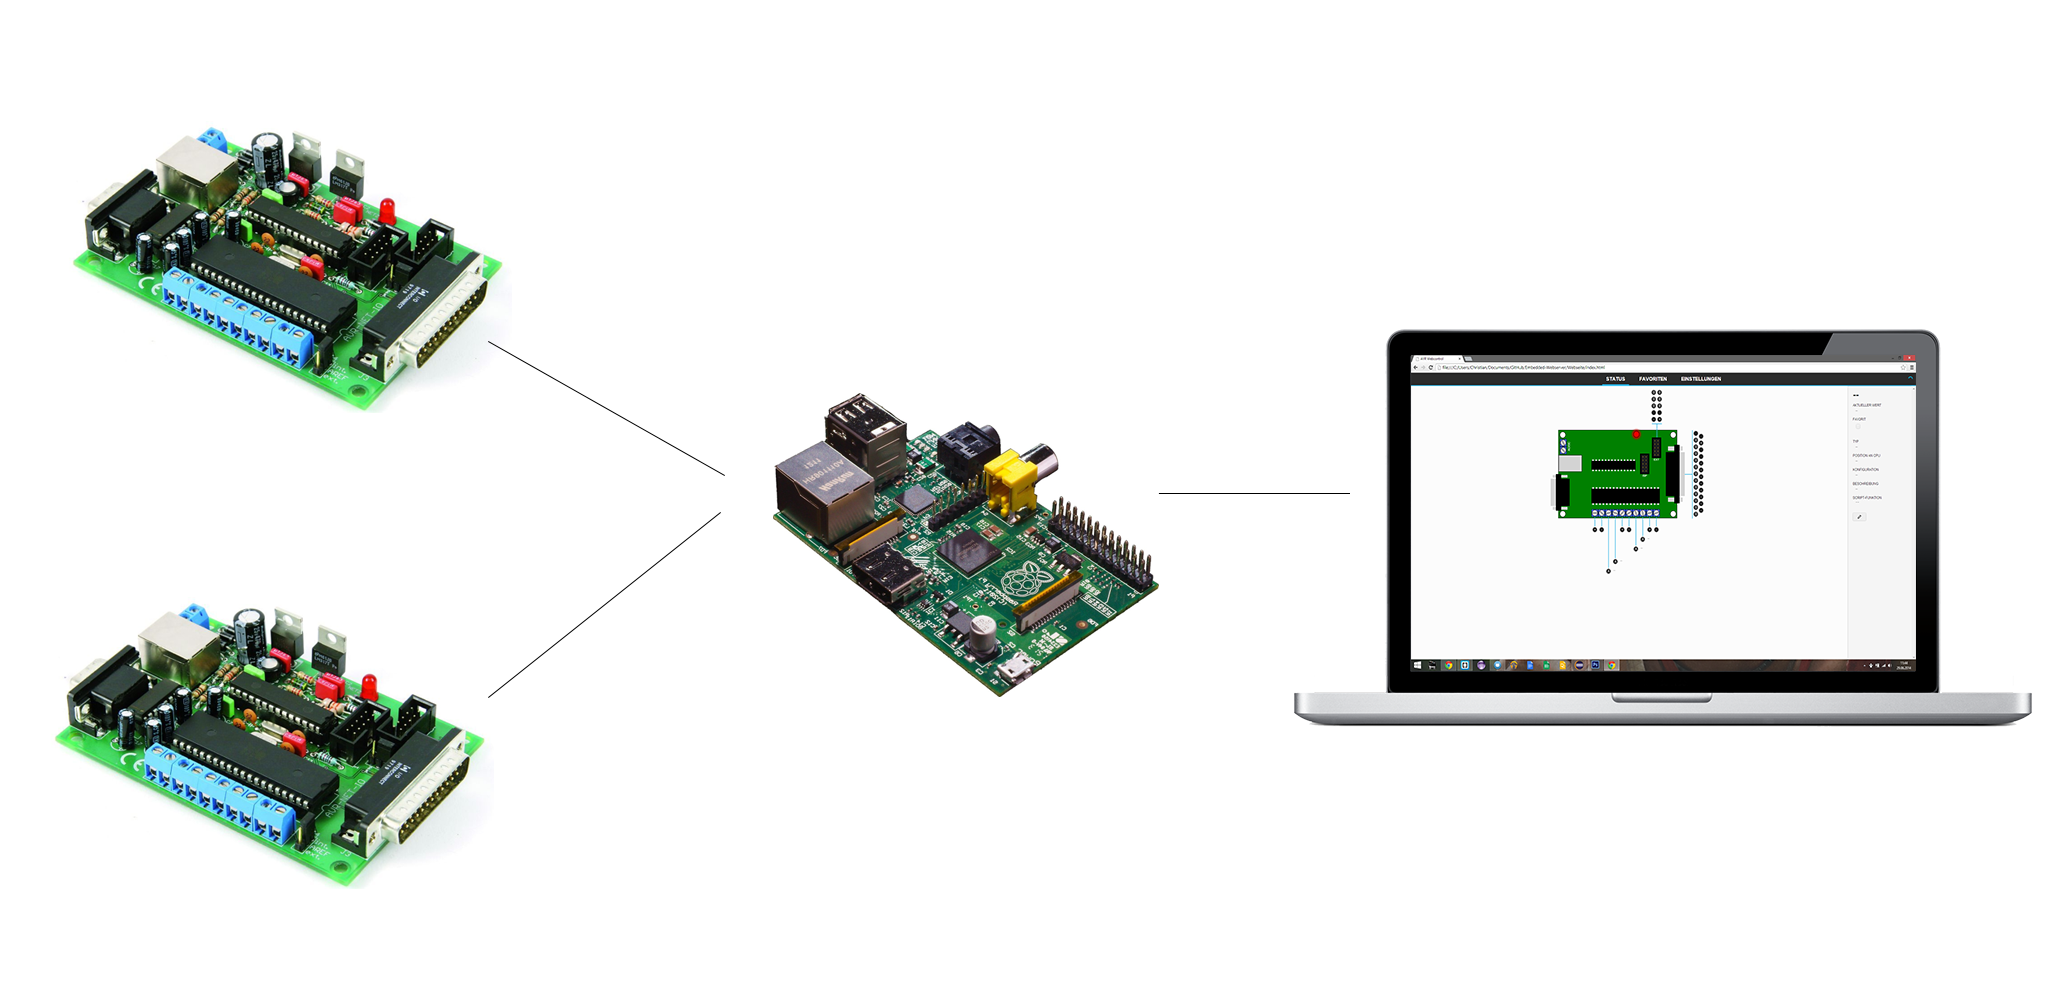
\includegraphics[width=13cm]{content/pictures/neues_system.png}
\caption{Der grobe Aufbau des neues Systems, links zwei Pollin Net-IO Boards,
in der Mitte ein Rasberry Pi und links ein Client}
\label{ausbau1}
\end{figure}
Die Clients fragen alle Daten, welche in einer kleinen Datenbank
zwischengespeichert werden sollten, von dem zentralen Rasberry Pi ab. So ergeben
sich zwei Teilsysteme. \\
\\
Das erste besteht aus dem Rasberry Pi und den Pollin Net-IO Boards,
welche über die von Pollin bereit gestellte Schnittstelle kommunizieren.
Die verwendung der bereits vorhandenen Schnittstelle macht es unnötig am
Microcontroller irgendwelche Änderungen vorzunehmen oder eine neue Firmware
flashen zu müssen, was die Usability enorm steigert, da das System auch von
Laien betrieben werden kann. Sobald neue Werte vorliegen sollten die Pollin
Net-IO Boards die Änderungen zum Rasberry Pi pushen, welcher die Werte in einer
kleinen Datenbank zwischenspeichert.Zur Verwendung des bestehenden Protokolls 
muss dieses mit Wireshark analysiert und reverse engineered werden. Hierfür 
kann die Netzwerkkommunikation des Pollin Net-IO Boards mit der mitgeliferten 
PC-Software beobachtet werden.\\
\\
Das zweite System besteht aus dem Rasberry Pi und den Clients. Die Clients
fragen über HTTP beim Server die Webseiten-Dateien und Messwerte ab. Die
Messwerte sollten nicht wie bei der aktuellen Lösung gepollt sondern nur bei
bedarf mit Hilfe der im Kapitel Technischer Hintergrund erläuterten HTML5
Server-Sent Events Technik zum Client gepusht werden. Dies reduziert den
unnötigen Netzwerkverkehr. Ein Client kann immer nur ein Pollin Net-IO board
darstellen, deshlab muss dem Nutzer auf der Webseite die Möglichkeit gegeben
werden das darzustellende Board auszuwählen. Außerdem muss auf der Webseite die
zu verwendenden Boards (also welche der Rasberry Pi anspricht und den Clients
anbietet) konfiguriert werden können. Ansonsten ist die Webseite ohne große
Änderungen übernehmbar.

%-----------------------------------------------------------------------------------------
\section{Änderungen an der Webseite/Server-Schnittstelle}
Die Kommunikation zwischen Server und Webseite muss für die neuen Anforderungen
entsprechend erweitert werden. \\
\\
In einem ersten Schritt sollten alle REST-URLs um einen Parameter erweitert
werden, der das Pollin Net-IO Board identifiziert, von dem die Informationen
angefordert werden. Dies ist nötig, da das System über mehrere Boards
verfügen könnte.Der Parameter kann als HTTP-GET Parameter übergeben werden. Als
ID eignet sich z.B. die IP-Adresse des betreffenden Boards oder eine künstliche 
ID in Form einer fortlaufend höheren Zahl. Die aufzurufende URL wäre folglich
z.B. \textrm{/rest/values?id=192.168.2.6}.\\
\\
Danach sollte das aktuell über die POST-Parameter stattfindende
Setzen von Pins ebenfalls über die REST-Schnittstelle gelöst werden. Hierfür
müssen zwei neue URLs eingeführt werden, eine zum setzen der Pinwerte und eine
zum setzen des DDR Registers. Natürlich müssen auch die neuen URLs über den
Parameter zum identifizieren des betroffnen Boards verfügen.\\
\\
Zum Schluss muss noch eine URL bereitgestellt werden um eine Liste aller
verfügbaren Boards abfragen zu können. Zusätzlich muss noch eine URL zum
hinzufügen eines neuen Boards und eine zum entfernen eines vorhandenen Boards
angelegt werden.\\
\\
Sobald an der Webseite die Schnitstelle manipuliert wird, ist die Kommunikation
mit dem von uns entwickelten Server nicht mehr möglich. Das System kann nicht
mit HTTP-GET Parametern umgehen. Aus diesem Grund sollte zu Beginn der
Entwicklung ein Testserver aufgesetzt werden. Dieser kann aus einem lokalen
XAMPP-Server bestehen, welcher statt dynamisch Dateien für die
REST-Schnittstelle zu erzeugen über statische Dateien verfügt welche mit
Testwerten gefüllt sind. So würde z.B. unter \textrm{/rest/pininfo} eine reale
Datei liegen, in der anstatt der Platzhalter feste Werte eingetragen sind. Dies
ermöglicht die Entwicklung der Webseite bzw. dem Ansprechen des Servers ohne
einen funktionsfähigen Rasberry Pi.

%-----------------------------------------------------------------------------------------
\section{Änderungen an der Webseite}
\subsection{Einstellungen}
Die meisten Änderungen der Webseite finden in den JavaScript Dateien statt. Alle
Einstellungen werden mit Hilfe von \textrm{db.js} gespeichert. Aktuell werden
die Einstellungen lokal gespeichert. Dies kann entweder beibehalten werden oder
die Einstellungen können zentral auf dem Rasberry gespeichert werden, was es
ermöglichen würde Favoriten etc. zwischen mehreren Clients zu synchronisieren.
Hierfür müsste nur der Speicherort geändert werden, an dem \textrm{db.js} die
Daten ablegt. Anstatt diese lokal zu speichern müssten sie zum Server geschickt
werden, welcher sie wiederrum an alle anderen Clients weiterleitet.

\subsection{Implementierung der neuen Schnittstelle}
Die neue Schnittstelle zwischen Server und Webseite muss natürlich implementiert
werden. Alle hierfür nötigen Änderungen finden in der \textrm{rest.js} statt.
Neben der Implementierung der Server-Sent Events um neue Messwerte zu
Empfangen müssen auch neue Getter und Setter angelegt werden, um z.B. alle
vorhandenen Boards abfragen zu können.\\
\\
Aktuell wird die Funktion \textrm{refreshValues()} dazu verwendet, die Daten
zyklisch nachzuladen. Gestartet wird dieser Vorgang von 
\textrm{startNewRefreshTask()}. Diese Funktionen können in Folge der Umstellung
auf Server-Sent Events komplett gelöscht werden. Wichtig ist hierbei, das die
Fuktion \textrm{setOnValuesChanged()} und das Attribut
\textrm{onValuesChanged} beibehalten wird. Indem \textrm{onValuesChanged()}
aufgerufen wird, wird \textrm{ui.js} darüber informiert, das sich die Messwerte
geändert haben, was zur aktualisierung der Oberfläche führt.

\subsection{Scriptfunktionen}

\subsection{Auswahl des darzustellenden Boards}

\subsection{Verwaltung der Boards im System}

%-----------------------------------------------------------------------------------------
\section{Der neue Server}


%-----------------------------------------------------------------------------------------
\section{Herangehensweise an das Projekt}
